\documentclass[11pt, a4paper]{article}
% \usepackage[T1]{fontenc}
\usepackage[utf8]{inputenc}
\usepackage{listings}
\usepackage[margin=1.0in]{geometry}
\usepackage{color}
\usepackage{graphicx}
\usepackage{tabularx}
\usepackage{url} 

\title{Rock the net}
\author{Elias Frantar}
\author{Samuel Schmidt}
\author{Nikolaus Schrack}
\author{Gary Ye}
\date{\today{}, Wien}
\begin{document}

\lstset{ %
  backgroundcolor=\color{white},   % choose the background color; you must add \usepackage{color} or \usepackage{xcolor}
  basicstyle=\footnotesize,        % the size of the fonts that are used for the code
  breakatwhitespace=false,         % sets if automatic breaks should only happen at whitespace
  breaklines=true,                 % sets automatic line breaking
  captionpos=b,                    % sets the caption-position to bottom
% commentstyle=\color{mygreen},    % comment style
  deletekeywords={...},            % if you want to delete keywords from the given language
  escapeinside={\%*}{*)},          % if you want to add LaTeX within your code
  extendedchars=true,              % lets you use non-ASCII characters; for 8-bits encodings only, does not work with UTF-8
% frame=single,                    % adds a frame around the code
  keepspaces=true,                 % keeps spaces in text, useful for keeping indentation of code (possibly needs columns=flexible)
% keywordstyle=\color{blue},       % keyword style
% language=bash,                   % the language of the code
  morekeywords={*,...},            % if you want to add more keywords to the set
  numbers=left,                    % where to put the line-numbers; possible values are (none, left, right)
  numbersep=5pt,                   % how far the line-numbers are from the code
  numberstyle=\tiny\color{mygray}, % the style that is used for the line-numbers
  rulecolor=\color{black},         % if not set, the frame-color may be changed on line-breaks within not-black text (e.g. comments (green here))
  showspaces=false,                % show spaces everywhere adding particular underscores; it overrides 'showstringspaces'
  showstringspaces=false,          % underline spaces within strings only
  showtabs=false,                  % show tabs within strings adding particular underscores
  stepnumber=1,                    % the step between two line-numbers. If it's 1, each line will be numbered
  stringstyle=\color{mymauve},     % string literal style
  tabsize=2,                       % sets default tabsize to 2 spaces
  title=\lstname                   % show the filename of files included with \lstinputlisting; also try caption instead of title
}


\maketitle
\newpage
\tableofcontents
\newpage

\section{Task description}
% TODO
\section{Design}
% TODO
% 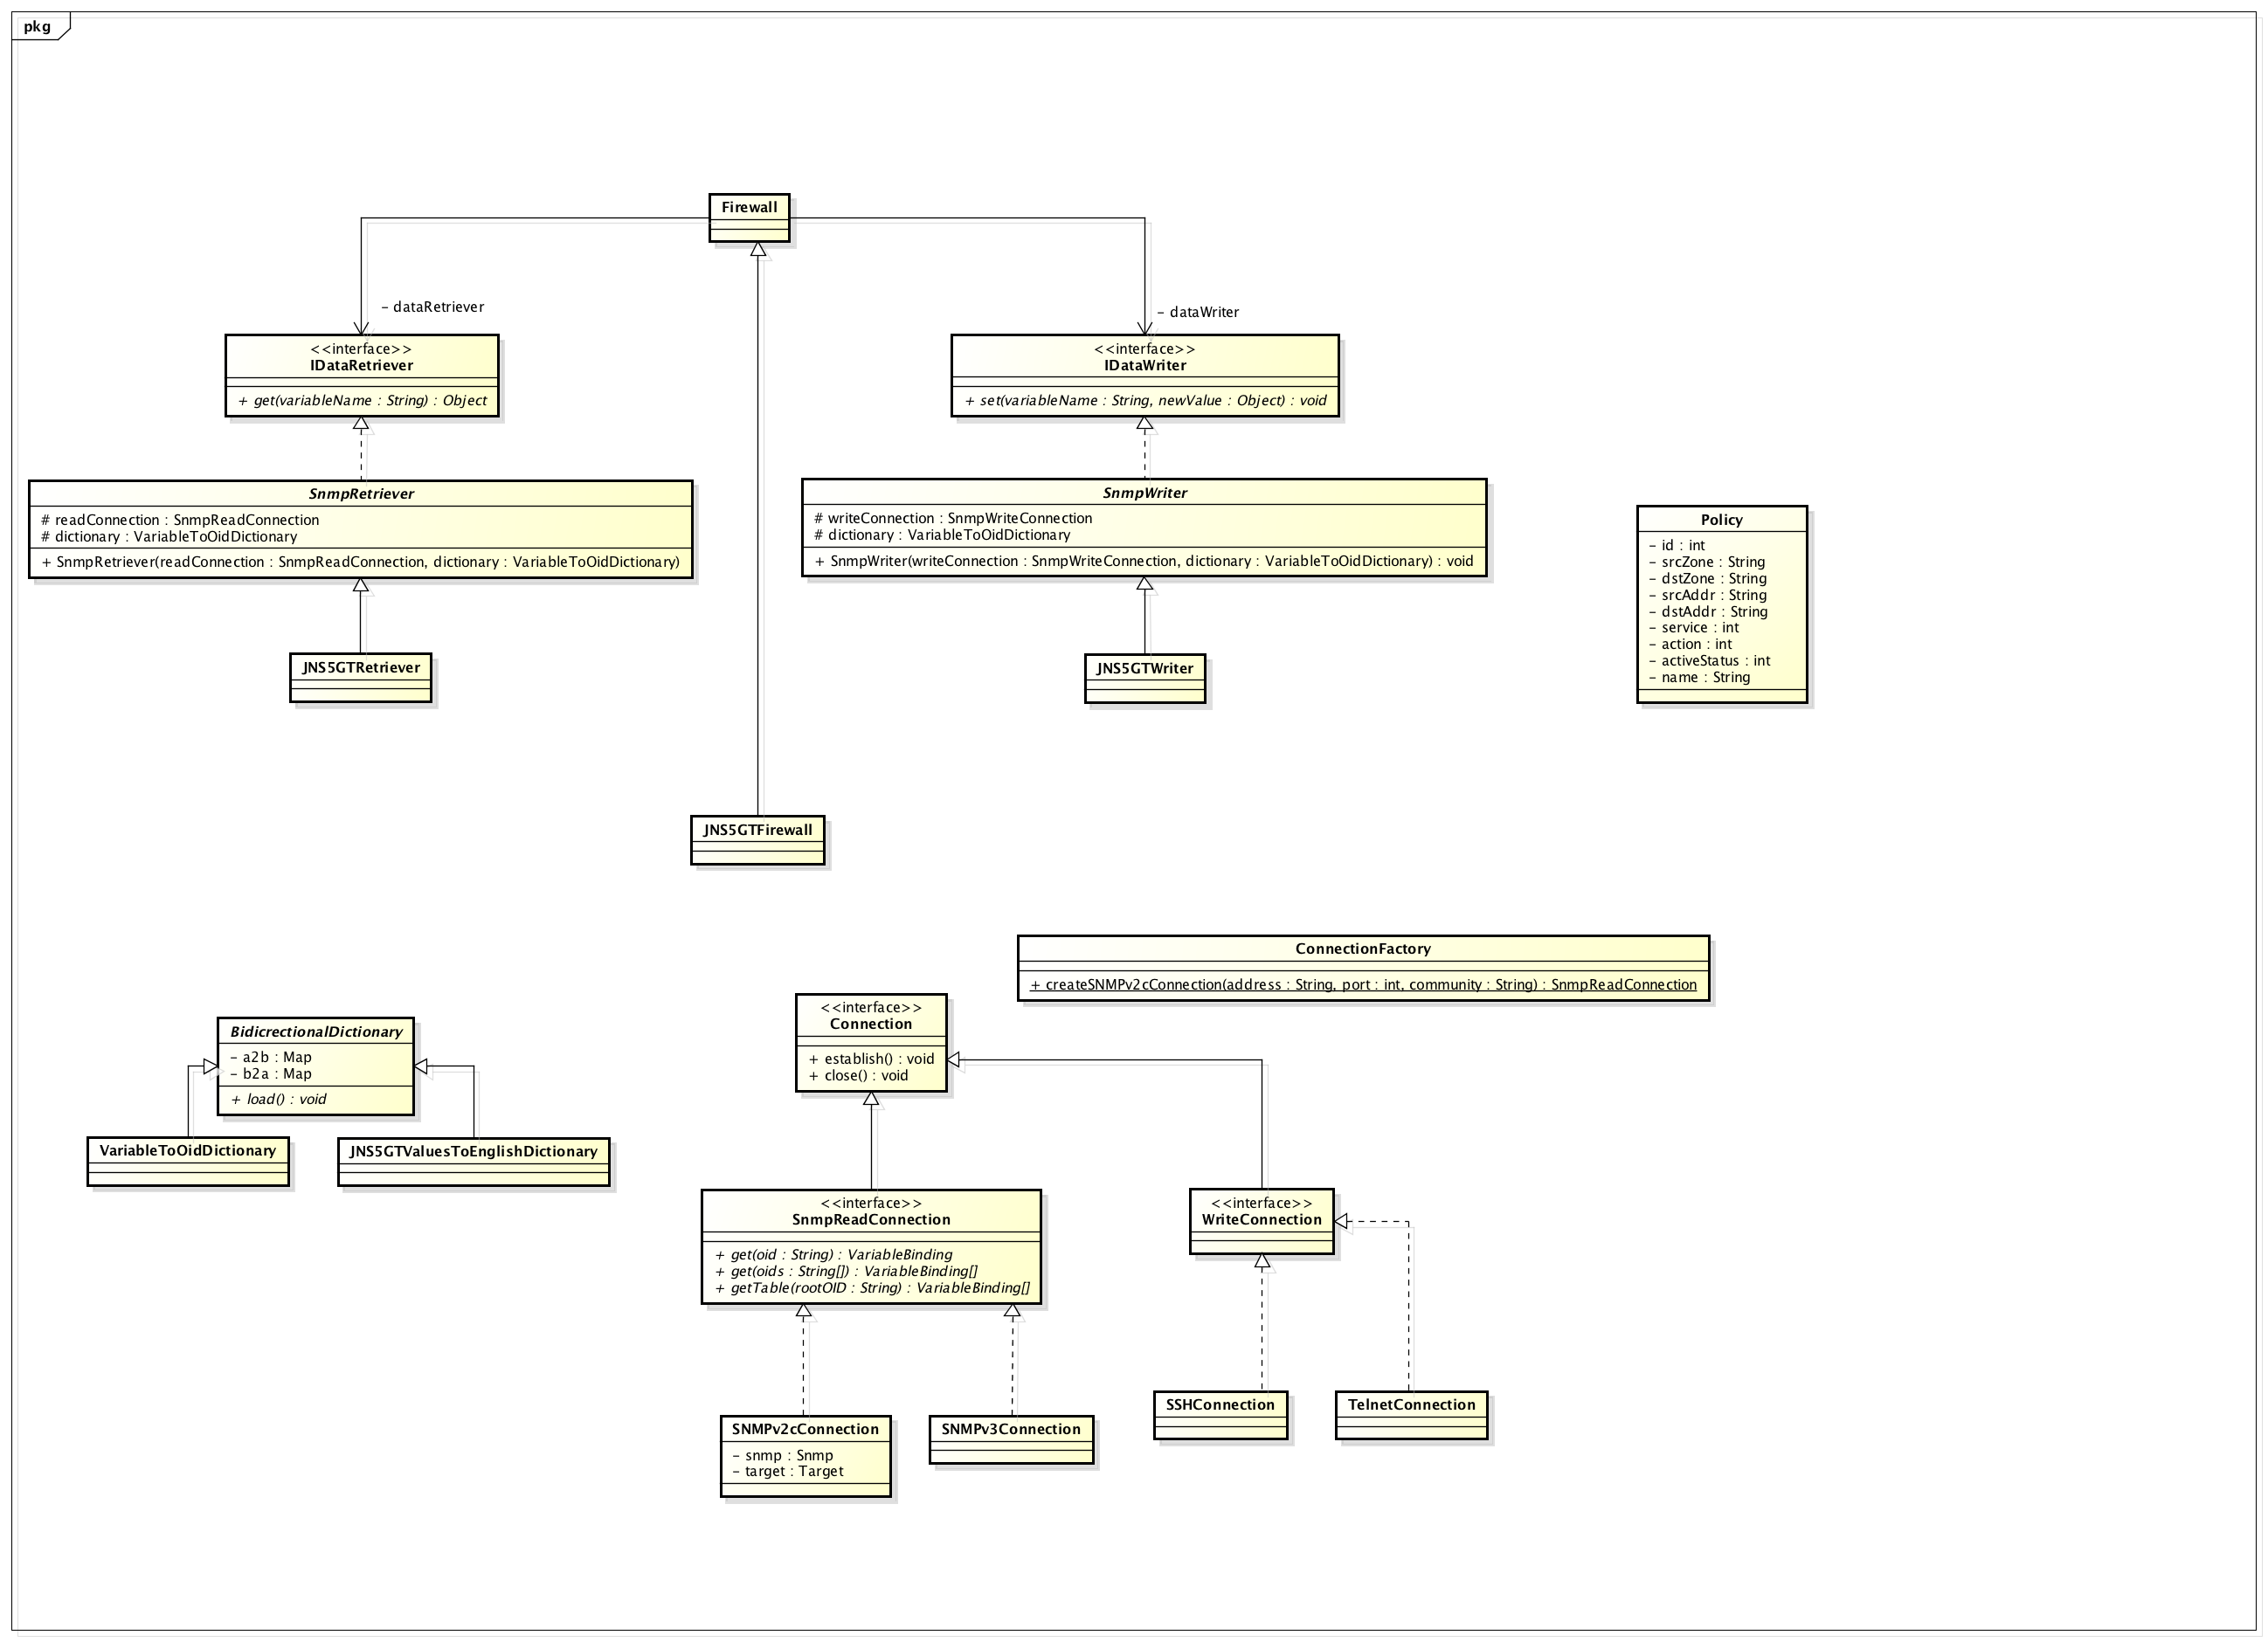
\includegraphics[width=\textwidth]{images/uml}
 
\section{Effort estimation}

Task	Original Estimate 	Remaining Estimate	Time spent
Preperation for the Tasks	20	0.00	24.50
List all configured firewall rules (policies) on the device, add the details of the mentioned services and zones as well.	7	2	9.50
Allow refreshing of the list by clicking a button and by a configurable time-intervall. Your GUI should remain responsive even with short refresh-intervals!	6	6	0.00
"Visualize the thru-put for a highlighted firewall-rule (nice2have: multiple rows) in a line-chart (configurable refresh-interval, unit bytes/sec)
"	8	4	5.00
Encapsulate the data retrieval for further reuse and easy expansion. An UML-model of your design will help you defend it at the review!	4	0.00	4.00
Build a visual appealing and easy to use interface (there is more than Swing out there).	10	7	8.00
Final Documentation 	8	12	5.00
Basic Total	63	31.00	56.00
Advanced Tasks			
Alarm the user visually and per email if the config of the firewall-rules changes. To avoid polling use the SNMP-trap mechanism.	7	5	0
Allow managing of firewall-rules (CRUD). To accomplish this, you will have to send configuration commands via telnet or ssh. An admin-account is available per request.	6	8	0
Use multicast-groups to build a simple transaction system to serialize administrative tasks on the firewall (for example pass an “admin token” to recognize the collaborator who is allowed to write to the firewall). This should also work in a heterogenous environment (different implementations, different OSes), so you have to coordinate with other teams.	8	15	0
Make sure, that your interface to the firewall allows an easy change of the firewall-model (new releases, manufacturer, ...). It is not necessary to make this configurable in the GUI but must (explicitly) be considered in your software-design!	5	0	2
Advanced Total	26	28	2
Total	89	59.00	58.00

\section{Installation}

\section{Technologies}
\subsection{Mock-Objects}
\subsection{Java FX}
\subsection{SNMP}
\subsubsection{Connection}
\subsubsection{MIBs}
\subsection{Multicast-Groups}

\section{Test report}
\section{Occurred problems}
\bibliography{protokoll}{}
\bibliographystyle{plain}
\end{document}
